\documentclass[10pt, twocolumn]{article}

%math
\usepackage{amsmath}
\usepackage{amssymb}
\usepackage{mathtools}
%logic
\usepackage{pgffor}
\usepackage{ifthen}
%science
\usepackage{siunitx}
\usepackage[version=4]{mhchem}
%language
\usepackage[english]{babel}
%formatting
\usepackage[a4paper, portrait, margin=1in]{geometry}
\usepackage{cuted}
\usepackage[small]{titlesec}
\usepackage[hidelinks]{hyperref}
\usepackage{parskip}
%images and plots
\usepackage{graphicx}
\usepackage[justification=centering]{caption}
\usepackage{subcaption}
\usepackage{float}
\usepackage{pgf}
\usepackage{import}
\usepackage{tikz}
\usepackage{jsonparse}
%tables
\usepackage{booktabs}
\usepackage{makecell}
%citation, quatation and lists
\usepackage[style=numeric,maxcitenames=2,sorting=none,doi=false,
url=false,isbn=false,eprint=false]{biblatex}
\usepackage[noabbrev,nameinlink]{cleveref}
\usepackage{csquotes}
\usepackage[nottoc]{tocbibind}
\usepackage{acro}


%setup plugins
\addbibresource{literature.bib}

\captionsetup{justification=centering}
\hypersetup{colorlinks=true,linkcolor=blue}


\DeclareSIUnit\angstrom{\text {Å}}
\DeclareSIUnit\bar{bar}
\sisetup{
	range-phrase = { to }
}

% Custom \citeauthoryear command with hyperref -> Rost et al. (2019) 
\DeclareCiteCommand{\citeauthoryear}
{\boolfalse{citetracker}%
\boolfalse{pagetracker}%
\usebibmacro{prenote}}
{\ifciteindex
{\indexnames{labelname}\indexfield{year}}
{}%
\printtext[bibhyperref]{%
    \printnames{labelname}%
    \setunit{\addspace}%
    \printtext{(}%
    \printfield{year}%
    \printtext{)}}}
{\multicitedelim}
{\usebibmacro{postnote}}

%  setup custom commands
\newcommand{\imcite}[2][]{From \cite[#1]{#2}.}
\newcommand{\imcitetwo}[2][]{Based on \cite[#1]{#2}.}
\newcommand{\integral}[4]{\int_{#1}^{#2} #3 \mathrm{d} #4}
\newcommand{\derivative}[2]{\frac{\mathrm{d}}{\mathrm{d} #1} #2}

%import json





% Document
\begin{document}
\pagenumbering{arabic}
\begin{figure*}
    \centering
    \begin{subfigure}{0.3\linewidth}
        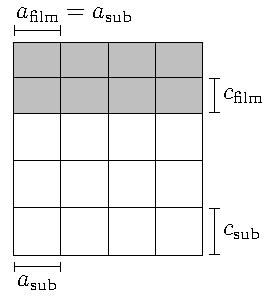
\includegraphics{../assets/pseudomorphic.pdf}
        \caption{Pseudomorphical growth of a thin film on a substrate}
    \end{subfigure}
    \begin{subfigure}{0.3\linewidth}
        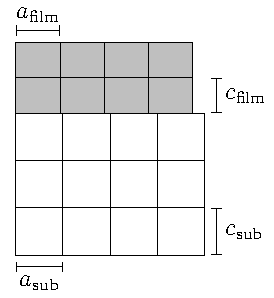
\includegraphics{../assets/partially_relaxed.pdf}
        \caption{Partially relaxed thin film on a substrate}
    \end{subfigure}
        \begin{subfigure}{0.3\linewidth}
        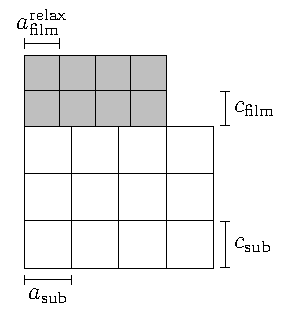
\includegraphics{../assets/fully_relaxed.pdf}
        \caption{Fully relaxed thin film on a substrate}
    \end{subfigure}
    \caption{(a) The unit cells of the substrate and the thin film are shown. The lattice constant 
    of the thin film is larger than that of the substrate. (b) The thin film is grown 
    pseudomorphically on the substrate. The in-plane lattice constant of the thin film is compressed 
    to match that of the substrate, while the out-of-plane lattice constant is expanded.}
\end{figure*}

\end{document}
